%==============================================================================
% Sjabloon poster bachproef
%==============================================================================
% Gebaseerd op document class `a0poster' door Gerlinde Kettl en Matthias Weiser
% Aangepast voor gebruik aan HOGENT door Jens Buysse en Bert Van Vreckem

\documentclass[a0,portrait]{hogent-poster}

% Info over de opleiding
\course{Bachelorproef}
\studyprogramme{toegepaste informatica}
\academicyear{2023-2024}
\institution{Hogeschool Gent, Valentin Vaerwyckweg 1, 9000 Gent}

% Info over de bachelorproef
\title{Competitief sportplatform met gamification zodat werknemers in een sedentaire job meer bewegen}
\subtitle{Een proof of concept}
\author{Sarah Eggermont}
\email{sarah.eggermont@student.hogent.be}
\supervisor{Sebastiaan Labijn}
\cosupervisor{Guillaume Vande Maele (we are)}

% Indien ingevuld, wordt deze informatie toegevoegd aan het einde van de
% abstract. Zet in commentaar als je dit niet wilt.
\specialisation{Mobile \& Enterprise developer}
\keywords{Gamification, sportplatform, gezondheid}
% \projectrepo{https://github.com/user/repo}

\begin{document}

\maketitle

\begin{abstract}

Beweging speelt een grote rol in zowel de fysieke als de mentale gezondheid van mensen. Bijna één derde van de wereldbevolking beweegt te weinig en ondervindt hier vroeg of laat de nadelen van. Om die reden bespreekt dit onderzoek of een sportplatform, dat gebruik maakt van gamification, gebruikt kan worden om medewerkers van \href{https://en.joule.be/}{Joule}, \href{https://www.ventures4growth.com/en}{Ventures 4 Growth}, \href{https://www.mace-legal.com/}{mace}, \href{https://planetb.life/en}{PlanetB}, \href{https://www.we-are.be/}{we are} en \href{https://www.delaware.pro/en-be}{delaware}, die een sedentaire job beoefenen, aan te zetten om meer te sporten.

Dit onderzoek suggereert dat een sportplatform met gamification wel degelijk zorgt voor een verbetering in de hoeveelheid beweging van mensen in een sedentaire job. Daarnaast stelt het dat gamificationtechnieken zoals punten en scoreborden, vooral wanneer dit zorgt voor een onderlinge competitie, het meest succesvol zijn. Tenslotte zijn er in dit onderzoek geen gamificationtechnieken opgemerkt die een negatief effect hebben op de hoeveelheid beweging van gebruikers, maar moet wel opgemerkt worden dat, binnen de context van een sportapplicatie, personen het storend vinden om meldingen te ontvangen als deel van de gamification.

\end{abstract}

\begin{multicols}{2} % This is how many columns your poster will be broken into, a portrait poster is generally split into 2 columns

\section{Introductie}

\subsection{Probleemstelling}
Een sedentaire job wordt geassocieerd met schadelijke gevolgen voor de algemene gezondheid. 31.1\% van de bevolking beweegt te weinig. Voorgaande onderzoeken hebben aangetoond dat een sportplatform met spelelementen kan helpen om mensen te motiveren meer te bewegen, echter bleek daar ook uit dat dit niet voor iedereen een motiverende factor is. Daarnaast is voor mensen in een sedentaire job nog geen bewijs gevonden dat ze hun zittend gedrag compenseren tijdens hun vrije tijd. Om deze redenen richt dit onderzoek zich op mensen in een zittend beroep.

\subsection{Onderzoeksvragen}

Deze paper zal de volgende onderzoeksvragen beantwoorden:

\begin{itemize}
    \item Heeft een competitief sportplatform, dat gebruik maakt van gamification, een positieve invloed op het sportgedrag van werknemers met een sedentaire job?
    \item Welke gamificationtechnieken hebben het meeste succes?
    \item Zijn er technieken die een negatief effect hebben?
\end{itemize}

\section{Methodologie}

\begin{center}
    \captionsetup{type=figure}
    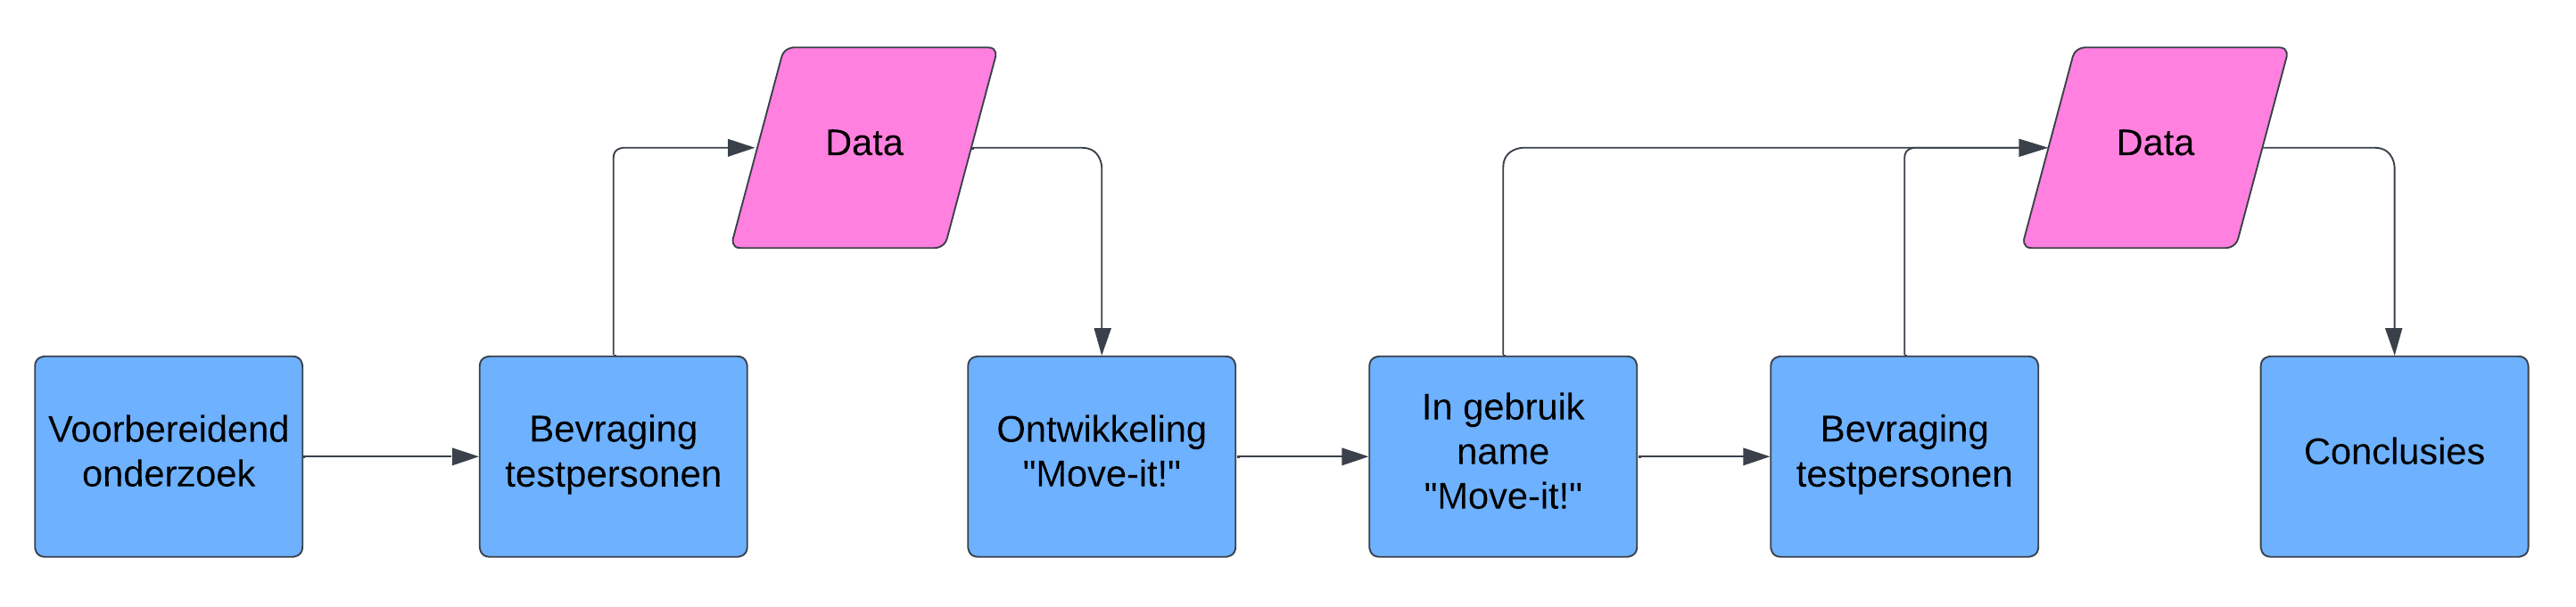
\includegraphics[width=1.0\linewidth]{Methodologie}
    \captionof{figure}{Flowchart van de gehanteerde methodologie.}
\end{center}

\section{Resultaten}

Slechts één van de acht consistente deelnemers behaalt de minima, voorgeschreven door de ``World Health Organization'' (WHO), niet sinds het gebruiken van het ontwikkelde sportplatform: ``Move-it!''. Daarnaast is bij 62.5\% van de deelnemers een stijging merkbaar in de hoeveelheid beweging sinds het gebruiken van ``Move-it!''.

\begin{center}
    \captionsetup{type=table}
    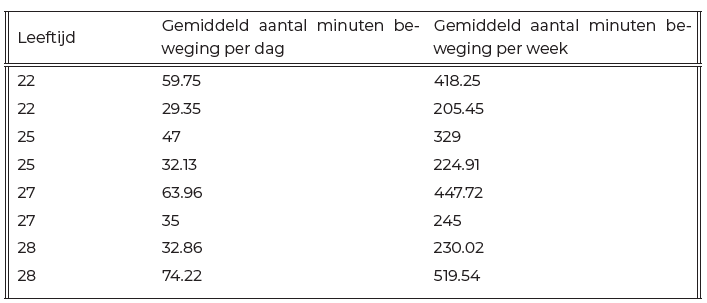
\includegraphics[width=.8\linewidth]{Beweging}
    \captionof{table}{Gemiddeld aantal minuten beweging per dag en per week van de meest consistente deelnemers.}
\end{center}

Wanneer mensen aangeven waarom ze minder bewegen dan ze zouden willen, komen volgende punten naar boven: te weinig tijd, geen motivatie, wederkerende blessures en geen plezier in sporten.

\begin{center}
    \captionsetup{type=figure}
    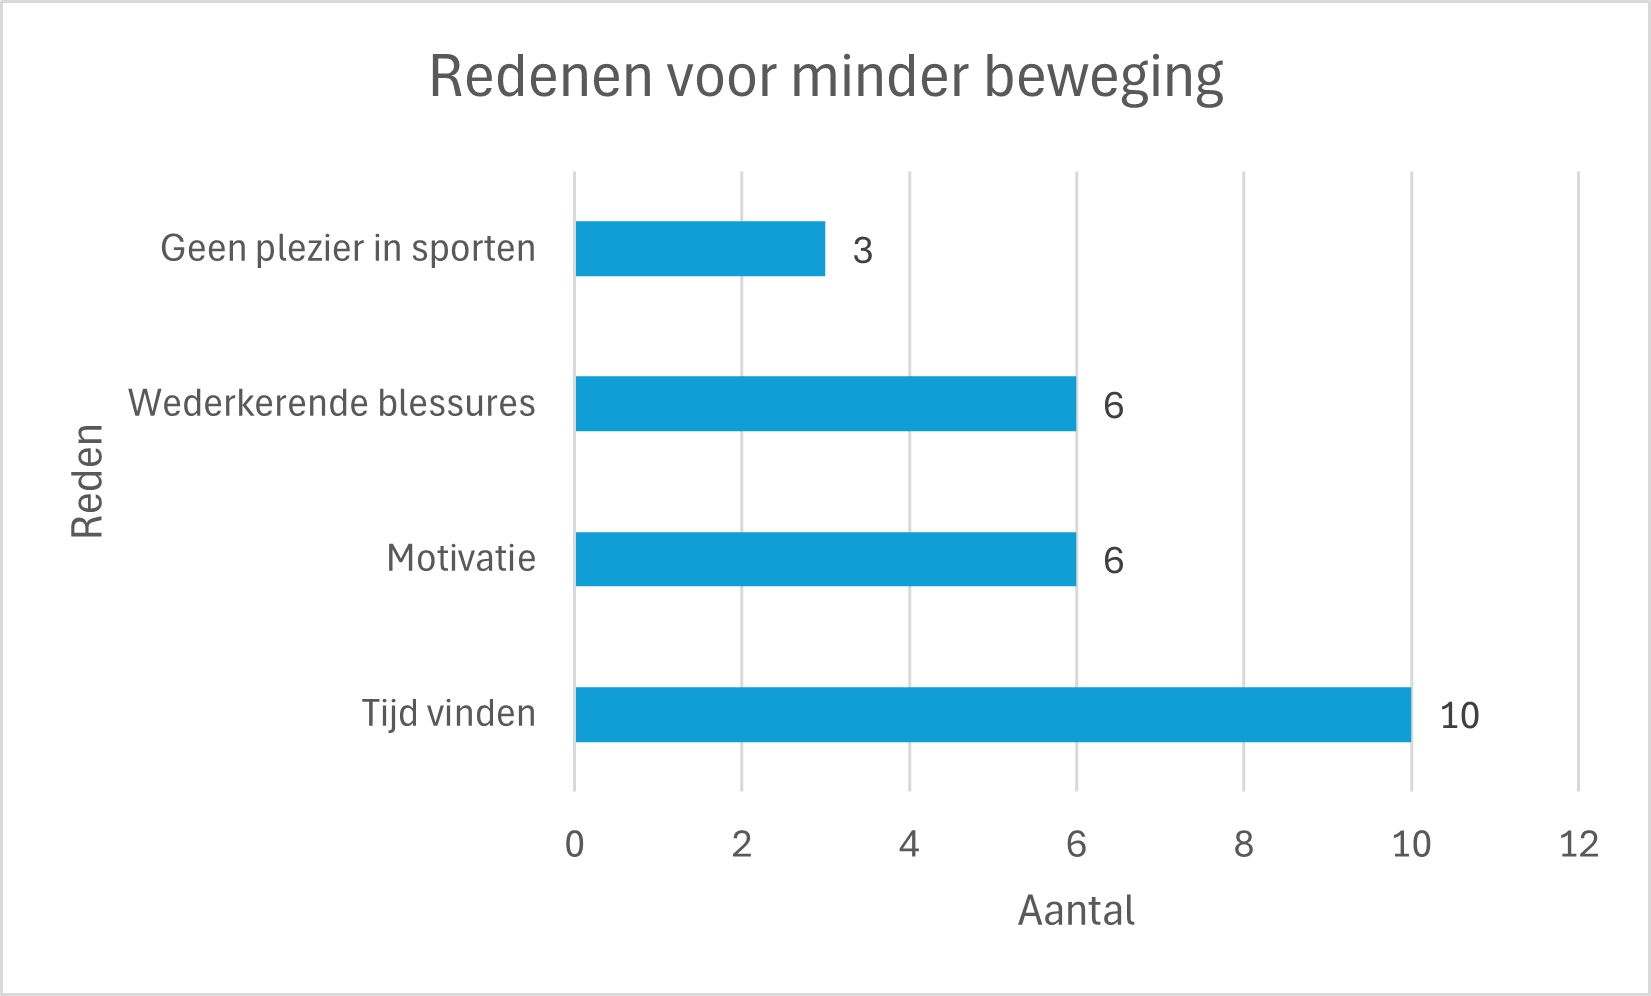
\includegraphics[width=.8\linewidth]{Waarom}
    \captionof{figure}{Redenen waarom deelnemers minder bewegen dan ze zouden willen.}
\end{center}

\section{Conclusies}

Deze paper suggereert dat een competitief sportplatform, dat gebruik maakt van
gamification, een positieve invloed heeft op het sportgedrag van werknemers met een sedentaire job.

Op vlak van gamification, hebben punten en scoreborden het meeste succes, vooral wanneer dit zorgt voor een onderlinge competitie. Er zijn in dit onderzoek geen gamification technieken naar boven gekomen die een negatief effect hebben op de hoeveelheid beweging. Specifiek voor sportapplicaties, suggereert dit onderzoek echter wel dat gebruikers het storend vinden om meldingen te ontvangen als deel van de gamification. In welke mate dit een mogelijke beslissende factor is in het al dan niet gebruiken van een sportapplicatie, moet verder onderzoek uitwijzen.

\section{Beperkingen huidig onderzoek}

Gezien het beperkte aantal deelnemers, moeten de bekomen resultaten en conclusies met voorzichtigheid benaderd worden en kunnen ze niet veralgemeend worden voor alle personen met een sedentaire job.

\section{Toekomstig onderzoek}

Een eerste aanbeveling voor verder onderzoek, is het vergroten van de
steekproef. Daarnaast leiden ook de volgende onduidelijkheden of vragen tot verder onderzoek:

\begin{itemize}
    \item Zijn de resultaten verschillend wanneer er een onderscheid gemaakt kan worden tussen intensieve activiteiten en activiteiten met gemiddelde intensiteit?
    \item Geven personen die weinig maar wel intensief sporten enkel deze gegevens in, waardoor het lijkt dat ze minder doen dan mensen die regelmatig minder intensief bewegen? Of bewegen ze effectief weinig naast deze intensieve activiteiten?
    \item Welk effect heeft een sportplatform met gamification voor mensen van 45 jaar of ouder?
\end{itemize}


\end{multicols}
\end{document}